\begin{figure*}[!th]
    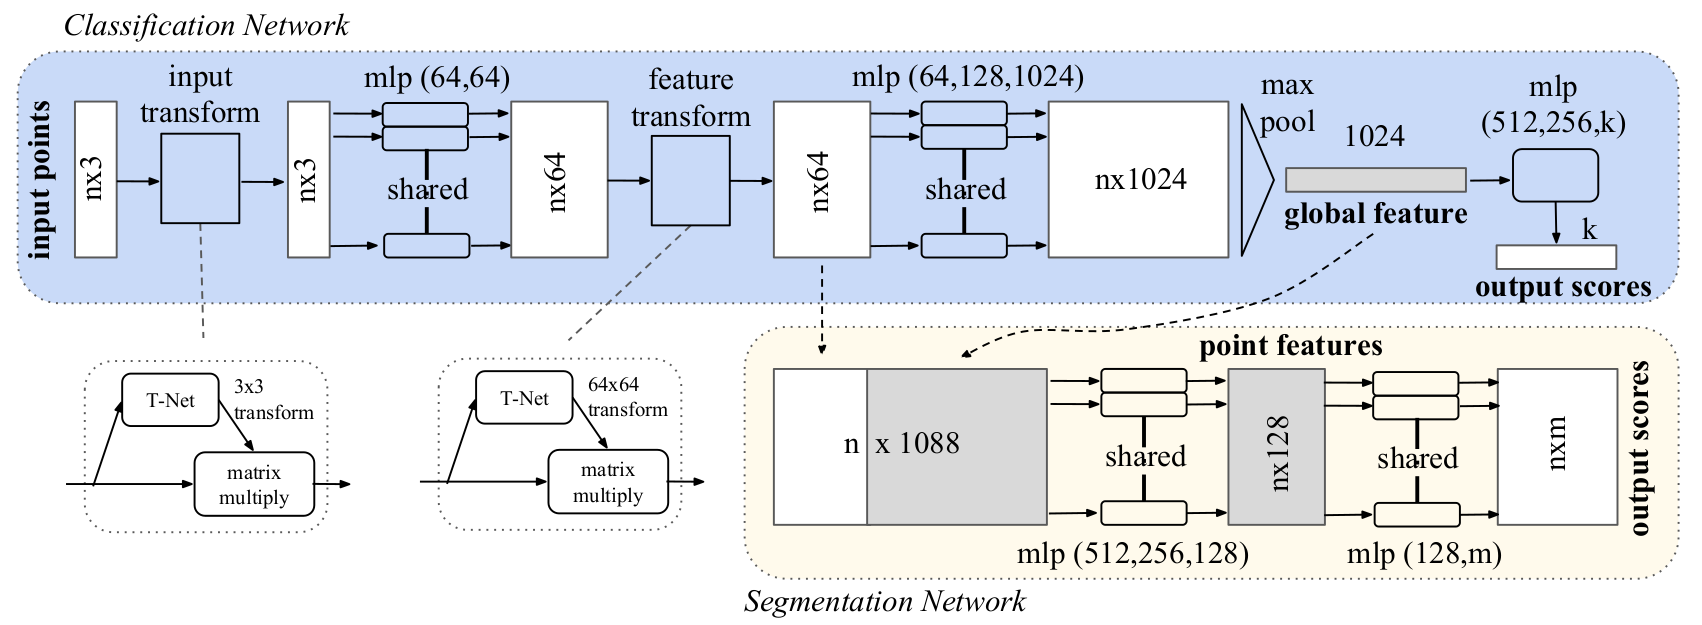
\includegraphics[width=\textwidth]{pointnet_architecture}
    \caption{
        \textbf{Architecture of PointNet.}
        The classification network takes $n$ points as input, applies input and
        feature transformations. Local features are aggregated to global
        features by max pooling, and reduced to classification scores for $k$
        classes as output. The segmentation network is an extension that
        concatenates global and local features and outputs per point scores.
        ``mlp'' describes a multi-layer perceptron. Numbers in brackets are
        layer sizes. All layers with ReLU use batchnorm. Dropout layers are
        used for the last mlp in classification net.
        % "The classification network takes $n$
        % points as input, applies input and feature transformations, and then
        % aggregates point features by max pooling. The output is classification
        % scores for $k$ classes. The segmentation network is an extension to the
        % classification net. It concatenates global and local features and
        % outputs per point scores. “mlp” stands for multi-layer perceptron,
        % numbers in bracket are layer sizes. Batchnorm is used for all layers
        % with ReLU. Dropout layers are used for the last mlp in classification
        % net." Figure and caption taken from \cite{qi2017pointnet}. \todo{rewrite in own words}
        Figure from \cite{qi2017pointnet}.
    } \label{fig:architecture}
\end{figure*}
